\documentclass[11pt,a4paper]{article}

\usepackage[T1]{fontenc}
\usepackage{lmodern}
\usepackage[margin=1in]{geometry}
\usepackage{amsmath,amssymb}
\usepackage{booktabs}
\usepackage{array}
\usepackage{graphicx}
\usepackage{pgfplots}
\pgfplotsset{compat=1.18}
\usepackage[hidelinks]{hyperref}
\usepackage{xcolor}
\usepackage{caption}
\captionsetup{font=small,labelfont=bf}

\title{\bfseries Can an AI proof loop replace model checking?\\[0.4em]
\large A measured comparison of TLC against machine-closed Lean proofs\\[0.2em]
\normalsize with wall-clock and dollar costs}

\author{Gavin Mendel-Gleason\and Maren Roos}
\date{\today}

\begin{document}
\maketitle

\begin{abstract}
\noindent
Model checking a TLA\textsuperscript{+} specification with TLC is push-button and exhaustive, but only
over a \emph{bounded} instance: it answers ``no violation up to $N$''. A proof answers ``for all $N$'',
and until recently the cost of obtaining one was human-weeks. We ask whether an AI proof loop --- a
language model driving Lean~4 through a shell until a mechanically checked closure oracle accepts the
artifact --- can close that gap, and at what cost.

Across four concurrent algorithms (token-ring mutual exclusion, Lamport's Bakery, LCR leader election
and EWD998 termination detection) the loop closed every task's general theorem, each with a negative
control demonstrating that the rig detects a weakened model. \textbf{The headline claim is supported on
4 of 4 tasks: the loop proves the general theorem inside a 2\,h / \$50 budget, its worst cell median
using 6.2\% of the clock and 0.0012\% of the money, where TLC cannot answer at any budget.}
\textbf{The same-claim cost comparison is withdrawn.} Every tier-2 median, and two of the tier-1 arms,
rest on rows whose transcripts show prior-proof reuse; re-earning those six cells under per-package
isolation produced thirty attempts of which \emph{five of six} arms again contained a prior-proof read,
because the attempt's shell still reaches the repository's templates and results even when its own package
holds no prior proof. That is a result about running a priced AI proof loop, and it is reported here in
place of a table built on contaminated samples. On a fresh Paxos cell --- the task whose general theorem
and bounded instance are the same claim --- the loop settled the general statement in a strict majority of
five attempts with \emph{no} proof failures, at a median of 1640.7\,s and \$0.00472. A tier-1 corollary
pilot at the same instance adds 267.3\,s, so the same-claim proof total is \textbf{1908.0\,s} against
TLC's \textbf{1405.9\,s} --- and because the corollary term cannot be negative while every measured
instance costs less and the next one cannot be exhausted inside the budget, \textbf{the crossing is
nonviable} for every instance TLC completes. That \emph{supports} H1 rather than leaving its crossover
unmeasured, and it is the pre-registered prediction under H1.

We report the method, the four tasks, the measured matrix, and at length what the result does
\emph{not} establish.
\end{abstract}

\section{Introduction}

TLC decides a bounded instance by enumeration. That is the right instrument for a design under
development, and its limitation is structural rather than a matter of speed: it cannot establish an
invariance for arbitrary $N$, and its cost grows exponentially in the instance size. Theorem provers
answer the general question, but the published human effort is substantial. The TLA\textsuperscript{+}
Trifecta paper~\cite{trifecta} reports \textbf{one person-day} for an invariance proof of EWD998, and
the IJCAR 2010 TLAPS papers~\cite{tlaps-ijcar} report proof-line counts in the hundreds with no time
figure at all.

Three developments make the question worth asking now: reasoning models that can plan proof steps,
Lean~4~\cite{lean4} with Mathlib~\cite{mathlib} as a target whose kernel is small and whose libraries
are broad, and --- the part we emphasise --- the ability to \emph{verify} a candidate proof mechanically
rather than trust the model that produced it. Recent work measures how often such models can prove
benchmark problems~\cite{deepseek-prover-v2,kimina-prover,goedel-prover}. We measure something
different: what a \emph{closed} theorem costs in wall-clock and dollars, against the model checker it
would replace, on the same specification.

Our question is therefore: \emph{can a loop close general theorems for concurrent systems, at what
wall-clock and dollar cost, and how does that compare with what TLC costs on the same claim?}

\section{Prior work}

Comparing TLC with proof on one specification is not new, and every published comparison pays for the
proof in human time. The TLA\textsuperscript{+} Trifecta paper~\cite{trifecta} applies TLC, Apalache and
TLAPS to EWD998: TLC finds 1.3 million distinct states in 42\,s at $N=3$ and 219 million in about
50 minutes at $N=4$, Apalache checks an inductive invariant at $N=100$ in 20\,s, and the TLAPS
invariance proof took one person-day and about 230 lines, with safety plus refinement at about 110 and
liveness at 245. Pastry~\cite{pastry} is the extreme case: TLC spent more than a month over
1\,952\,882\,411 states without a counterexample, and the authors conclude that interactive proof effort
``is too high to scale to more complete P2P protocols''. The IJCAR 2010 TLAPS papers~\cite{tlaps-ijcar}
report proof sizes with no time figure at all: Peterson about 130 lines, Bakery 800, Paxos 550 to
``somewhat over 1000''. Reports from industry have the same shape: ten AWS systems, specifications of
102--939 lines, two to three weeks of tool learning and 0--3 bugs each~\cite{aws}; seL4 at about
20 person-years and 480{,}000 lines of proof~\cite{sel4}. That a model checker settles an instance while
a proof settles the theorem is the standard framing of the two methods~\cite{clarke-wing}, and it is the
framing used here.

What has changed is the price of proof search. Work on AI provers measures how often a model closes
benchmark problems~\cite{deepseek-prover-v2,kimina-prover,goedel-prover}; it does not price a closed
theorem against the model checker it would replace, on the same specification. \textbf{No published work
compares an AI-driven proof loop's wall-clock and dollar cost against TLC's runtime for the same
specification}, and that is the comparison reported below.

The prior art those figures come from is committed here at pinned provenance: the EWD998 specification
with both TLAPS proofs (\texttt{tlaplus/Examples} at \texttt{3dfe0087}, \texttt{specs/tla/ewd998/}), the
IJCAR 2010 modules (\texttt{tlaplus/tlapm} at \texttt{7824dab5}, \texttt{specs/tla/ijcar2010/}), and the
publication-era revision of EWD998 that reproduces the published TLC figures
(\texttt{specs/tla/ewd998-paper/}). The imported proofs are \emph{not} machine-checked here ---
\texttt{tlapm} is not in the dev shell and is invoked nowhere in this repository --- so the effort
figures are cited data marked \texttt{machine\_checked: false}, never a measured arm (\S5.3). Two
disagreements between the published counts and the committed artifacts are recorded rather than
reconciled.

\section{Method}

\subsection{Two routes, two tiers}

\textbf{Route~A} is TLC enumerating a TLA\textsuperscript{+} specification at a bounded instance.
\textbf{Route~B} is a Lean~4 theorem closed by an AI proof loop.

Each task has two Route~B tiers. \textbf{Tier~2} is the general theorem: the property for arbitrary
$N$. \textbf{Tier~1} is that theorem's corollary, instantiated at the calibrated instance $N_0$. Only
tier~1 is comparable with Route~A, because only tier~1 proves the same claim.

$N_0$ is fixed by a stated rule: \textbf{the largest $N$ whose TLC run completes inside the 2\,h
per-run cap.} That definition is what fixes EWD998's $N_0$ (\S5.1).

\subsection{The closure criterion}

A \emph{closed} verdict comes from three checks run by code the candidate cannot reach:

\begin{enumerate}
\item \textbf{Integrity} --- the candidate is byte-identical to the seed up to and including the
      theorem's \texttt{:=}. This pins every definition and the statement; only the proof body is free.
\item \textbf{Elaboration} --- the candidate is handed to \texttt{lean} directly, with no \texttt{lake}
      in the invocation. The candidate has a shell and can reach the package's lakefile, so a
      lake-built environment would be \emph{the candidate's}, not the harness's.
\item \textbf{Closure} --- a prebuilt checker imports the elaborated olean and reads the declaration's
      axiom set out of Lean's \emph{API}, against
      $\{\texttt{propext},\ \texttt{Classical.choice},\ \texttt{Quot.sound}\}$.
\end{enumerate}

The third is load-bearing and its implementation matters. \texttt{\#print axioms} is \emph{syntax},
syntax is an environment extension a candidate can install, and it crosses imports --- in testing, a
candidate rewrote the command into text of its own and the real report never ran. An API query cannot
be reached that way. Both attacks that defeated the first form of this check --- a candidate printing a
fake axiom report, and a candidate redefining \texttt{\#print axioms} in its own syntax --- were found
by an independent reviewer rather than by the loop, and both now fail closed.

Around those three: the bytes checked are one immutable snapshot taken once per round and never
re-read, so the verdict, the result row and the durable closure copy all derive from the same bytes;
the elaboration environment is captured before the session opens; and the seed's digest is re-checked
on every exit path.

\subsection{Why a rate, not a run}

Closure is stochastic. The unit of evidence is therefore a \textbf{cell}: $R \ge 5$ runs sharing one
seed digest, never pooled across configurations. The complement is the \textbf{negative control} ---
the loop is run against the task's \emph{mutant}, a weakened model, and must \emph{fail} to close it.
Without that, a working prover and a broken rig are indistinguishable.

\subsection{Measurement}

We record wall-clock, peak RSS, dollar cost from provider usage at list price, and distinct states
enumerated. Route~A runs at its best measured configuration with the row naming it, and worker count is
reported because it moves wall-clock but not state counts.

\section{The task set}

\begin{table}[htbp]
\centering
\small
\begin{tabular}{@{}lll@{}}
\toprule
Task & Property & Source \\
\midrule
token-ring & mutual exclusion & our bootstrap model \\
Bakery & mutual exclusion & Lamport~\cite{bakery} \\
LCR & at most one leader & Le Lann~\cite{lelann}, Chang \& Roberts~\cite{changroberts} \\
EWD998 & termination detection (invariance) & Dijkstra~\cite{ewd998}; imported with the proofs of~\cite{trifecta} \\
\bottomrule
\end{tabular}
\caption{The four tasks. EWD998 is externally calibrated: both the specification and the published
TLAPS proofs are imported at pinned provenance, and the human-effort figures attach to it.}
\end{table}

\section{Results}

\subsection{The measured matrix}

\begin{table}[htbp]
\centering
\small
\begin{tabular}{@{}lrrrr@{}}
\toprule
 & \textbf{token-ring} & \textbf{Bakery} & \textbf{LCR} & \textbf{EWD998} \\
\midrule
Route~A $N_0$                       & 23 & 9 & 10 & 3 \\
Route~A wall-clock                  & 837.9\,s (8 workers) & 4{,}847.7\,s & 2.7\,s & 36.4\,s \\
Route~A cost                        & \$0.04655 & \$0.26932 & \$0.00015 & \$0.00202 \\
Route~A distinct states             & 289{,}406{,}976 & 238{,}803{,}200 & 177{,}147 & 1{,}520{,}618 \\
\midrule
\textbf{tier 2} (general $N$)       & \textbf{closed} 104.8\,s & \textbf{closed} 444.4\,s & \textbf{closed} 216.0\,s & \textbf{closed} 162.0\,s \\
tier-2 cost                         & \$0.00033 & \$0.00062 & \$0.00044 & \$0.00047 \\
\textbf{tier 1} (corollary)         & \textbf{closed} 38.5\,s & \textbf{closed} 76.6\,s & \textbf{closed} 101.0\,s & \textbf{closed} 112.3\,s \\
tier-1 cost                         & \$0.00023 & \$0.00048 & \$0.00042 & \$0.00051 \\
\midrule
negative control                    & TLC \texttt{violation} & \texttt{fail\_to\_close} & \texttt{fail\_to\_close} & \texttt{fail\_to\_close} \\
\bottomrule
\end{tabular}
\caption{The measured matrix. Tier-2 figures are medians over the runs that closed, each quoted with
its closure count against non-mutant attempts: $6/8$, $5/7$, $5/5$, $5/5$ for token-ring, Bakery, LCR
and EWD998 (tier~1: $7/8$, $5/5$, $5/5$, $6/6$). The five non-closures are three provider faults, one
budget \texttt{timeout}, and one unclosed run whose row records no kind; mutant controls are separate
runs and never attempts. Ranges are wide --- token-ring's spans 62.9--1021.8\,s --- so no figure is
quoted without its range. Route~A at $N_0$ is a single deterministic run except EWD998, whose six runs
give the median shown. \textbf{Withdrawn as cost measurements:} the four tier-2 cells and the Bakery and
LCR tier-1 cells rest on rows whose transcripts show prior-proof reuse, and the re-earned reruns failed
their audit gate as well (\S5.5). The counts and medians above are historical observations, not
independent samples.}
\end{table}

\noindent
EWD998's $N_0 = 3$ is the cap's value rather than a convergence artifact. Its instance search first
looked like one: every failing invocation of $N=4$--$6$ carried TLC's \texttt{-cleanup}, which deletes
the state pool mid-enumeration, and without it \textbf{$N{=}4$ completes} --- 248{,}006{,}200 distinct
states, depth 104, 2\,h\,36\,min, exit~0. That clean run finishes outside the 2\,h per-run cap, so the
stated rule of \S3.1 selects $N_0 = 3$ on its own authority: removing the flag changed the ground of the
value, not the value. The flag is also not a general cause of failure --- Bakery reached 238{,}803{,}200
distinct states and token-ring 289{,}406{,}976 \emph{with} it in place.

\subsection{Same-claim cost, counted honestly}

A corollary is the trivial instantiation of its theorem, so the corollary's cost alone answers ``what
does instantiation cost \emph{given} the theorem''. The question asked is what \emph{settling the
claim} costs, which is theorem plus corollary:

\begin{table}[htbp]
\centering
\small
\begin{tabular}{@{}lrrrrrr@{}}
\toprule
Task & Route~A & theorem & corollary & \textbf{proof total} & \textbf{$K$} & favours \\
\midrule
token-ring ($N{=}23$) & 837.938\,s & 104.8\,s & 38.5\,s & \textbf{143.4\,s} & \textbf{0.171} & proof, 5.8$\times$ \\
Bakery ($N{=}9$)      & 4{,}847.749\,s & 444.4\,s & 76.6\,s & \textbf{521.0\,s} & \textbf{0.107} & proof, 9.3$\times$ \\
EWD998 ($N{=}3$)      & 36.4\,s & 162.0\,s & 112.3\,s & \textbf{274.3\,s} & \textbf{7.53} & \textbf{TLC, 7.5$\times$} \\
LCR ($N{=}10$)        & 2.670\,s & 216.0\,s & 101.0\,s & \textbf{317.0\,s} & \textbf{118.7} & \textbf{TLC, 118.7$\times$} \\
\bottomrule
\end{tabular}
\caption{$K = \text{proof} \div \text{TLC}$ on the same claim. On cost the
totals are kinder to the proof --- cheaper on three of four; only LCR favours TLC on both resources.
\textbf{These totals are withdrawn.} Every tier-2 median, and the Bakery and LCR tier-1 arms, rest on rows
with prior-proof reuse; the re-earned reruns failed their audit gate (\S5.5), so no recomputed $K$ is
published and \textbf{no split is a result}.}
\end{table}

\begin{figure}[htbp]
\centering
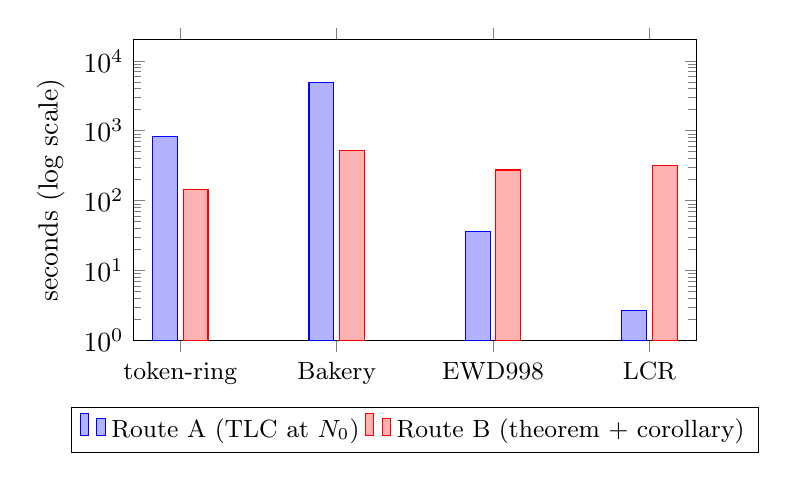
\begin{tikzpicture}
\begin{axis}[
  width=0.72\textwidth, height=5.4cm,
  ybar, bar width=9pt,
  ylabel={seconds (log scale)}, ymode=log,
  symbolic x coords={token-ring,Bakery,EWD998,LCR},
  xtick=data, x tick label style={font=\small},
  legend style={font=\small, at={(0.5,-0.22)}, anchor=north, legend columns=-1},
  ymin=1, ymax=20000,
]
\addplot coordinates {(token-ring,837.938) (Bakery,4847.749) (EWD998,36.4) (LCR,2.670)};
\addplot coordinates {(token-ring,143.4) (Bakery,521.0) (EWD998,274.3) (LCR,317.0)};
\legend{Route A (TLC at $N_0$), Route B (theorem $+$ corollary)}
\end{axis}
\end{tikzpicture}
\caption{The same claim, both routes, log scale. \textbf{The routes trade places rather than one
dominating}: the loop is cheaper on token-ring (5.8$\times$) and Bakery (9.3$\times$), TLC is cheaper on
EWD998 (7.5$\times$) and LCR (118.7$\times$). Which way a task falls follows its calibration, not the
methods: every $N_0$ is the instance the rule of \S3.1 selected --- and for LCR the 2\,h cap never bound,
so the sweep's extent set it --- rather than the instance where the two routes cross. A task calibrated
so that both routes are under pressure at the same instance is the experiment this plot shows is still
missing. \textbf{The totals plotted are the withdrawn ones of \S5.2}: what survives is the \emph{shape}
--- exponential against flat --- not the values.}
\end{figure}

\subsection{Against published human effort}

\begin{table}[htbp]
\centering
\small
\begin{tabular}{@{}lll@{}}
\toprule
Our task & Human comparator & Reported \\
\midrule
\texttt{ewd998} & TLAPS invariance & \textbf{1 person-day}, $\sim$230 lines \\
\texttt{ewd998} & TLAPS safety $+$ refinement & \textbf{0.5 person-day}, $\sim$110 lines \\
\texttt{ewd998} & TLAPS liveness & \textbf{$<$1 person-day}, 245 lines \\
\texttt{ijcar2010-*} & TLAPS proofs & lines only --- \textbf{no time reported} \\
token-ring, Bakery, LCR & \textbf{none published} & --- \\
\bottomrule
\end{tabular}
\caption{Cited data, never a measured arm: the human figures are imported with quotes and pinned
provenance, marked \texttt{machine\_checked: false}, and never pooled with either route.}
\end{table}

\noindent
Only EWD998 has a published person-day figure, so the human comparison is one number against one
number: a person-day against EWD998's \textbf{274.3\,seconds} of loop time (theorem plus corollary),
the widest of the four tasks' totals being Bakery's \textbf{521.0\,seconds}, and every total
\textbf{under 1.5 millidollars}. The IJCAR papers report lines, and we do not convert lines into days.

\subsection{The verdict, against each reading of ``replacement''}

\begin{table}[htbp]
\centering
\small
\begin{tabular}{@{}>{\raggedright\arraybackslash}p{0.30\textwidth}>{\raggedright\arraybackslash}p{0.62\textwidth}@{}}
\toprule
Reading & Result \\
\midrule
\textbf{General theorem inside budget $B$} &
\textbf{Supported, 4 of 4.} Worst cell median 444.4\,s $=$ \textbf{6.2\%} of the 2\,h cap, and the
largest tier-2 cost \$0.00062 $=$ \textbf{0.0012\%} of the \$50 cap. TLC's coverage of this tier is
0 of 4 at any budget. \\
\addlinespace
\textbf{Cost parity at the bounded tier ($K$)} &
\textbf{Withdrawn}: the cell medians behind $K$ rest on rows with prior-proof reuse, and the re-earned
reruns failed their audit gate (\S5.5), so no split is reported. \\
\addlinespace
\textbf{Coverage under a fixed budget} &
Counts equal at 4 of 4, claims not equal: the loop settles four \emph{general} theorems; TLC settles
four \emph{bounded} instances and zero of the general tier. \\
\bottomrule
\end{tabular}
\caption{Protocol readings of what ``replacing model checking with proof'' might mean, each reported
rather than one chosen for the reader.}
\end{table}

\subsection{Paxos: the general theorem inside the budget, and what isolation does not fix}

\textbf{The theorem and the cell.} Paxos is the task the set was missing: one where the bounded instance
TLC can check and the general theorem the loop proves are the \emph{same claim} rather than neighbours.
The loop settled the general statement --- arbitrary acceptor count, arbitrary value type,
pairwise-intersecting quorums, unbounded ballots, no ballot bound and no fixed value set --- with the
retained proof of \texttt{Paxos.agreement} depending only on \texttt{propext},
\texttt{Classical.choice} and \texttt{Quot.sound}, and on no \texttt{sorryAx}. The measured cell ran five
attempts on one seed digest, each in its own prepared Lean package with its own workspace, results and
session root, file mode, one repetition per invocation. \textbf{Three of five attempts carry the final
verdict} --- a strict majority --- and \textbf{zero attempts failed to prove anything}: the two
non-certified attempts had clean integrity, elaboration, permitted axioms and an intact seed, and were
withheld for rig reasons only (one put a scratch file outside the allowed prefix; one lost its verdict to
an instrument fault, below). The all-attempt median is \textbf{1{,}640.690\,s} (range 386.999--1{,}716.946)
at a cell cost of \textbf{\$0.00472} (the five rows' own \texttt{cost\_usd} summed), with the withheld
attempts' actual elapsed times included --- the selection operand is never a median over closures only.

\textbf{What it licences, and why the crossing is settled rather than merely absent.} This median is one
of the two operands of the same-claim proof total $P(N) = \text{median}(\text{tier-2 theorem}) +
\text{median}(\text{tier-1 corollary at }N)$, and the other is now measured. A tier-1 corollary pilot at
the fixed six-acceptor instance --- the loop instantiating the proved general theorem, five attempts on one
seed digest, each in its own prepared package whose receipt lists \texttt{PaxosProved} as a dependency it
may see --- gives a clean-attempt median of \textbf{267.315\,s} --- 418.929\,s over all five, with the one
attempt that read a prior artifact of the same seed excluded rather than pooled --- so
\textbf{$P(6) = 1{,}908.005$\,s} against Route~A's measured \textbf{$A(6) = 1{,}405.943$\,s}. The corollary
therefore costs about a sixth of the theorem --- H2's ``instantiation is free'' made concrete --- and the
sum still exceeds the largest instance TLC completes. The corollary term cannot be negative, so $P(N) \ge 1{,}640.690$\,s for every $N$, while
every measured $A(N) \le 1{,}405.943$\,s and the next candidate has no successfully exhausted row at all:
the crossing's second conjunct fails at every candidate, so \textbf{the crossing is nonviable}, and no
further corollary measurement can change it. That \emph{supports} H1 rather than leaving a gap in it ---
for every instance TLC completes, the proof route costs more --- with H2's crossover lying beyond the
pinned family, which is the pre-registered prediction under H1. \texttt{n\_cap} and \texttt{n\_0} remain
null, now for a settled reason rather than a missing operand. The comparison is also conservative in the
claim's favour: the corollary instantiates the general theorem with unbounded $\mathbb{N}$ ballots, while
the bounded TLC row it is priced against checks a single-ballot projection, so the priced pair is not two
measurements of one claim and the figure above is not flattered by the difference. Both cells are
exploratory pilots, and neither is \textbf{pooled} with the earlier five-row Paxos pilot, whose oracle
certified a decoy declaration and whose repetitions copied each other's proofs: that pilot is retained as
diagnostic, and its single independent datum was 1{,}934.76\,s. Nothing here is a Route~A/Route~B ratio and
nothing here should be divided by another task's total.

\textbf{A result about the rig, which stands on its own.} Re-earning the six contaminated published arms
--- thirty attempts, each in its own prepared package whose receipt shows exactly what it could see ---
established that \textbf{per-package isolation is necessary and insufficient on a host with no read
sandbox}. Five of the six arms contained at least one attempt whose transcript shows a prior proof read,
by two routes: a tier-2 attempt read the \emph{shared template's} \texttt{<Task>Proved.lean} by absolute
path --- the package had correctly withheld that module, so what leaked was the \emph{reachable corpus},
not the package, and one attempt reached \emph{another task's} proof --- and a tier-1 attempt read prior
\emph{evidence}: a published cell's session transcript, a sibling attempt's result row, the prepare
receipts. Of thirty attempts, nineteen survived the audit and fifteen of those closed. The methodological
statement is not that the loop fails but that \textbf{a priced AI proof loop needs the attempt's reachable
corpus removed, not merely its own directory cleaned}: with no kernel boundary available here, a shell
that can name a path can read it, and the models name the paths unprompted, from their first attempt
onward. The cross-task cost tables are therefore withdrawn rather than replaced.

\textbf{The instrument the numbers rest on, and why it was replaced twice.} Every file-mode verdict
depends on a watch that reports writes outside the working copy, and its first form read
\texttt{inotifywait}'s own reassurance --- \texttt{Watching new directory <path>}, printed when the tool
\emph{adds} a watch --- as an unreadable stream, so a run that organised scratch into a subdirectory of the
one path it was allowed to write forfeited its verdict: the rig penalising compliance. Naming that message
benign then certified a write it never saw, because a path containing a newline splits a record across two
lines. The third form asks the tool for a machine-readable stream (\texttt{-q -c}), recognises only named
events, has \emph{no} exemptions, demonstrates its own watch with a nonce sentinel, and treats a reader
that dies --- an undecodable filename used to kill the reader silently --- as blindness rather than
silence. That sequence is the honest description of the numbers above.

\textbf{Caveats carried with this result.} The host load at the cell's launch was 2.26/2.15/1.71 on 20
cores, higher than the Paxos calibration cell's, so any wall-clock comparison across the two carries that
difference. Two mutation-arm attempts read a proof of the true model: their \emph{outcomes} stand as
negative controls and their wall-clock and dollar figures are not cost samples. And where this paper's
cross-task figures are compared against published ones, the comparison is \textbf{indicative}: those rows
predate the field that records a withheld verdict and were produced under a different verdict rule.

\section{Limitations}

These bound the claims, and we would rather state them than have them found.

\begin{enumerate}
\item \textbf{Different claims per row.} Route~A's row proves a bounded instance; Route~B's tier~2
      proves arbitrary $N$. Only the same-claim pairs of \S5.2 compare like with like.
\item \textbf{The equivalence is audited, not proved.} Lean-model $\equiv$
      TLA\textsuperscript{+}-semantics is a hand audit per task. A modelling slip would make the
      theorem true about the wrong thing.
\item \textbf{Model, not code.} Both routes prove properties of models; neither refines to an
      implementation.
\item \textbf{Safety only.} Liveness is out of scope. The published EWD998 figures split on exactly
      that line (1 person-day invariance, $<$1 person-day liveness).
\item \textbf{No pair was measured at a crossover.} Every $N_0$ came from the calibration rule of \S3.1
      --- the largest instance Route~A completes inside the 2\,h cap --- not from where the two routes
      trade places, and for LCR that cap never bound, so the sweep's extent stands in its place. That
      is \emph{why} \S5.2's pairs fall where they do; the split itself is now withdrawn (\S5.5). The cost
      shape (TLC exponential, proof flat) is measured; the crossover itself is extrapolated.
\item \textbf{Small task set.} Four algorithms, eight settled cells. Not a sampled population.
\item \textbf{Different precision across tasks.} Every cell has $R \ge 5$ closures on a single seed
      digest, but the counts differ --- LCR and EWD998 closed 5 of 5 non-mutant attempts, token-ring
      6 of 8 (one 2\,h \texttt{timeout}), Bakery 5 of 7 (two provider faults) --- and the quoted
      medians are over closures rather than pass rates over attempts. Since EWD998 anchors the human
      comparison, its 5 of 5 is the one that matters most.
\item \textbf{Stochastic costs.} Each row is one sample; verdicts are deterministic given an artifact,
      costs are distributions. Medians carry ranges for that reason.
\item \textbf{Cost basis.} Tokens at list price, compute at a stated host rate, researcher time not
      costed. Both components are reported separately and never merged.
\item \textbf{Our own tooling is young.} The closure oracle is software: the two attacks that defeated
      its first form (\S3.2) were found by review, not by the loop.
\item \textbf{The cross-task cost figures are withdrawn.} The published tier-2 medians for all four
      tasks, and two of the tier-1 arms, rest on rows whose transcripts show prior-proof reuse; the six
      affected arms were re-earned under per-package isolation and failed their audit gate as well, so no
      recomputed $K$ exists and \S5.2 reports none. The mutation-arm rows are usable as \emph{outcomes}
      and never as costs. Comparisons against the superseded published values are \textbf{indicative},
      because those rows predate the field that records a withheld verdict and were produced under a
      different verdict rule, and any wall-clock comparison carries the host-load difference recorded in
      \S5.5.
\end{enumerate}

\section{Conclusion}

An AI proof loop closes general theorems for real concurrent algorithms, at a cost of seconds to
seventeen minutes and under a millicent, inside a budget it barely touches --- the worst cell median
uses 6.2\% of the 2\,h clock and 0.0012\% of the \$50. \textbf{That answers a question TLC cannot be
asked} --- arbitrary $N$ rather than a bounded instance --- and it does so with a mechanically checked
artifact rather than a generated one.

It does not make model checking obsolete. On the same bounded claim, TLC is faster on two of four
tasks, and it checks the specification's semantics directly rather than a ported model whose
equivalence is a hand audit. \textbf{The honest summary is that the two routes answer different
questions at different costs, the crossover between them is the quantity that matters, and no
experiment yet measures it.} That is the obvious next step: a task calibrated so that both routes are
under pressure at the same instance.

\begin{thebibliography}{99}
\small

\bibitem{trifecta}
K.~Konnov, T.~Kuppe, and S.~Merz.
\newblock Specification and Verification With the TLA\textsuperscript{+} Trifecta: TLC, Apalache, and
TLAPS.
\newblock In \emph{ISoLA 2022}. \url{https://members.loria.fr/SMerz/papers/2022-isola.pdf}

\bibitem{tlaps-ijcar}
K.~Chaudhuri, D.~Doligez, L.~Lamport, and S.~Merz.
\newblock Verifying Safety Properties With the TLA\textsuperscript{+} Proof System.
\newblock In \emph{IJCAR 2010}. \url{https://members.loria.fr/SMerz/papers/ijcar2010.pdf}

\bibitem{lean4}
L.~de Moura and S.~Ullrich.
\newblock The Lean~4 Theorem Prover and Programming Language.
\newblock In \emph{CADE-28}, 2021.

\bibitem{mathlib}
The Mathlib Community.
\newblock The Lean Mathematical Library.
\newblock In \emph{CPP 2020}.

\bibitem{bakery}
L.~Lamport.
\newblock A New Solution of Dijkstra's Concurrent Programming Problem.
\newblock \emph{Communications of the ACM}, 17(8), 1974.

\bibitem{ewd998}
E.~W.~Dijkstra.
\newblock Derivation of a Distributed Termination Detection Algorithm.
\newblock EWD manuscript 998.

\bibitem{lelann}
G.~Le Lann.
\newblock Distributed Systems --- Towards a Formal Approach.
\newblock In \emph{IFIP Congress}, 1977.

\bibitem{changroberts}
E.~Chang and R.~Roberts.
\newblock An Improved Algorithm for Decentralized Extrema-Finding in Circular Configurations of
Processes.
\newblock \emph{Communications of the ACM}, 22(5), 1979.

\bibitem{deepseek-prover-v2}
DeepSeek-AI.
\newblock DeepSeek-Prover-V2: Advancing Formal Mathematical Reasoning via Reinforcement Learning for
Subgoal Decomposition.
\newblock arXiv:2504.21801.

\bibitem{kimina-prover}
Numina and Kimi teams.
\newblock Kimina-Prover Preview: Towards Large Formal Reasoning Models with Reinforcement Learning.
\newblock arXiv:2504.11354.

\bibitem{goedel-prover}
Goedel-LM.
\newblock Goedel-Prover: A Frontier Model for Open-Source Automated Theorem Proving.
\newblock arXiv:2502.07640.

\bibitem{pastry}
T.~Lu, S.~Merz, and C.~Weidenbach.
\newblock Towards Verification of the Pastry Protocol using TLA\textsuperscript{+}.
\newblock In \emph{FORTE 2011}. \url{https://members.loria.fr/SMerz/papers/forte2011pastry.pdf}

\bibitem{aws}
C.~Newcombe, T.~Rath, F.~Zhang, B.~Munteanu, M.~Brooker, and M.~Deardeuff.
\newblock How Amazon Web Services Uses Formal Methods.
\newblock \emph{Communications of the ACM}, 58(4):66--73, 2015.

\bibitem{sel4}
G.~Klein, K.~Elphinstone, G.~Heiser, J.~Andronick, D.~Cock, P.~Derrin, D.~Elkaduwe, K.~Engelhardt,
R.~Kolanski, M.~Norrish, T.~Sewell, H.~Tuch, and S.~Winwood.
\newblock seL4: Formal Verification of an OS Kernel.
\newblock In \emph{SOSP 2009}, pages 207--220.

\bibitem{clarke-wing}
E.~M.~Clarke and J.~M.~Wing.
\newblock Formal Methods: State of the Art and Future Directions.
\newblock \emph{ACM Computing Surveys}, 28(4):626--643, 1996.

\end{thebibliography}

\appendix
\section{Data provenance}

Every figure in \S5 is recomputable from rows committed in the repository; none is estimated. The
paper builds from \texttt{paper/model-or-proof.tex} through the repository's dev shell
(\texttt{nix develop -c latexmk -pdf}), so the artifact is produced from its source like everything
else here.

\begin{table}[htbp]
\centering
\small
\begin{tabular}{@{}>{\raggedright\arraybackslash}p{0.32\textwidth}>{\raggedright\arraybackslash}p{0.60\textwidth}@{}}
\toprule
Figure & Source \\
\midrule
Route~A rows & \texttt{results/tlc.jsonl}, with logs under \texttt{results/logs/} \\
Route~B rows & \texttt{results/proof.jsonl}; closure copies under \texttt{results/closures/<task>/} \\
Human comparators & \texttt{results/human.jsonl}; quotes pinned in \texttt{docs/human-baseline.md} \\
Method and decisions & \texttt{docs/protocol.md} \\
Closure criterion & \texttt{harness/closure\_oracle.py}, \texttt{tools/checker/PROVENANCE.md} \\
Equivalence audits & \texttt{docs/equivalence-\{token-ring,bakery,lcr,ewd998\}.md} \\
Full measured matrix & \texttt{wiki/comparison-matrix.md}, which also carries the two queries that
recompute \S5.1 and the Route~A rows \\
\bottomrule
\end{tabular}
\caption{Where each figure comes from. The matrix in \texttt{wiki/} exists so the numbers here can
be checked against the data rather than trusted as typeset.}
\end{table}

\end{document}
